\chapter{Bestehendes System}
\label{cha:basis}
Da die Arbeit bereits in ein bestehendes System integriert wird, gibt es Möglichkeiten, bereits vorhandenen Code wiederzuverwenden. Um die Implementierung (Kapitel \ref{cha:implementierung}) nachvollziehen zu können, werden in diesem Kapitel einzelne bestehende Konzepte vorgestellt, die dabei helfen, das Framework zu integrieren und weiterzuentwickeln.

\section{MVVM spezifische Erweiterungen}
\label{sec:mvvm_extensions}
Grundsätzlich basiert das WPF-System (siehe Unterabschnitt \ref{subsec:WPF}) auf dem in Unterabschnitt \ref{fig:mvvm_pattern} beschriebenen MVVM-Pattern. Würde jedoch die gesamte Logik direkt in die Vererbungshierarchie der ViewModels integriert werden, würde dies die Flexibilität erheblich einschränken und die Komplexität deutlich erhöhen. Daher wurde das MVVM-Pattern an die spezifischen Anforderungen der Anwendung angepasst.

\subsection{Presenter}
Bindings ermöglichen zwar einen relativ einfachen Datenaustausch zwischen View und ViewModel, jedoch treten häufig Situationen auf, in denen Daten das Verhalten der View beeinflussen oder Aktionen im ViewModel ausgelöst werden müssen, die sich über einfache Commands\footnote{Commands \cite{wpf_commanding_overview} sind ein Konzept, bei dem ein Objekt erstellt wird, das eine Aufgabe ausführt, wenn es getriggert wird. Dieses Objekt kann über ein Binding ausgetauscht werden.} nicht mehr abbilden lassen. 

In der betreffenden WPF-Anwendung kommen daher Presenter zum Einsatz, die die Kommunikation zwischen ViewModel und View sowohl auf Basis von Daten als auch über Events ermöglichen. Dem Presenter sind sowohl die View als auch das ViewModel bekannt, jedoch können weder View noch ViewModel auf den Presenter zugreifen.

Der Erzeugungsprozess des MVVM-Konstrukts mit Presenter sowie die beschriebenen Zusammenhänge sind in Abbildung \ref{fig:mvvm_with_presenter} dargestellt. Die dort abgebildete ViewModel Region ist ein Control, das die Darstellung eines ViewModels mithilfe der entsprechenden View vornimmt. Die ViewModel Region verwendet eine Factory, um die entsprechenden Presenter zu erzeugen. Die dazugehörigen Informationen, welche View und welcher Presenter für ein bestimmtes ViewModel erzeugt werden sollen, entnimmt die Factory der MVVM Config. 

Die grünen Pfeile in der Abbildung beschreiben den Datenaustausch über Bindings sowie die Events und Daten, die über den Presenter weitergeleitet werden können, wenn beispielsweise keine Commands oder kein verwendbares Binding zur Verfügung stehen.

\begin{figure}[H]
    \centering
    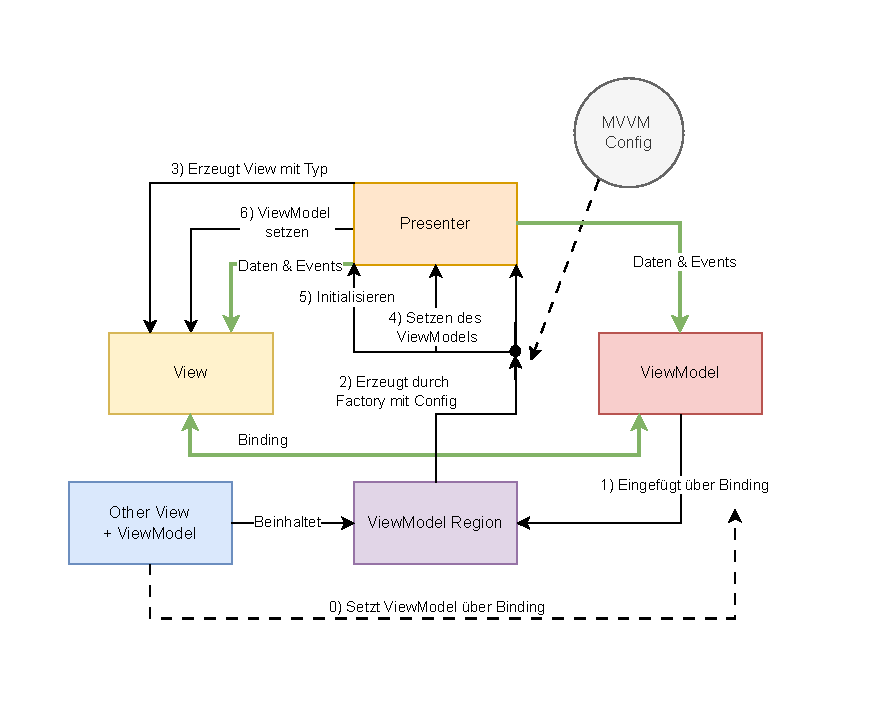
\includegraphics[width=0.8\textwidth]{4_Presenter_MVVM_Extension}
    \caption{Erstellungsprozess und Zusammenhänge des MVVM mit Presenter}
    \label{fig:mvvm_with_presenter}
\end{figure}

\subsection{ViewModel Extensions}
\label{subsec:viewmodel_extensions}
ViewModel Extensions erweitern ein ViewModel um zusätzliche Funktionalitäten, wie z.B. automatisches Speichern oder Datenvalidierung. Diese Erweiterungen werden für jedes ViewModel in einer Liste gespeichert und gemeinsam mit dem ViewModel initialisiert. Eine ViewModel Extension erhält Zugriff auf das ViewModel, das sie erweitert und kann über Properties des Haupt-ViewModels auch für das Binding zur View verwendet werden. ViewModel Extensions müssen dem ViewModel während des Konstruktionsprozesses hinzugefügt werden.

\subsection{Presenter und Presenter Extensions}
\label{subsec:presenter_extensions}
Presenter Extensions sind analog zu den zuvor beschriebenen ViewModel Extensions (siehe Unterabschnitt \ref{subsec:viewmodel_extensions}), erweitern jedoch den Presenter. Sie werden über eine Factory in der MVVM Config\footnote{Die MVVM Config ist eine Konfiguration, die die Zuordnung von ViewModel, View, Presenter und deren Extensions festlegt.} definiert. Dort können Presenter Extensions mit dem jeweiligen Presenter, der View, dem ViewModel und den zugehörigen ViewModel Extensions erzeugt werden. Presenter Extensions besitzen keine spezielle Struktur und müssen beim Erzeugen initialisiert werden. Wie auch ViewModels werden sie im entsprechenden Presenter gehalten.

\section{Windows Forms spezifische Erweiterungen}
\label{sec:mvp_extensions}
Wie auch in WPF (siehe Unterabschnitt \ref{subsec:WPF}) gibt es für Windows Forms (siehe Unterabschnitt \ref{subsec:Winforms}) einige Erweiterungen, welche die Entwicklung erleichtern und für die Integration des Frameworks in die Anwendung notwendig sind.

\subsection{Embedded Presenter}
\label{subsec:embedded_presenter}
In der mit Windows Forms (siehe Unterabschnitt \ref{subsec:Winforms}) umgesetzten Anwendung wird das MVP-Pattern strikt angewendet. Dennoch gibt es Aufgaben, die sich wiederholen und sich gut aus dem Hauptpresenter herauslösen lassen, um eine höhere Kohäsion zu erreichen. Für solche Aufgaben werden Embedded Presenter eingesetzt. Diese Presenter werden in einem Initialisierungsschritt im Hauptpresenter erzeugt und erhalten Zugriff auf diesen. Dadurch können typische Aufgaben wie Validierung, Speichern oder ähnliches ausgelagert sowie flexibel ausgetauscht oder ergänzt werden. Nach ihrer Erzeugung werden Embedded Presenter unmittelbar initialisiert.

\subsection{UI Accessor}

Um auf Events von Controls zugreifen zu können, wird der UI Accessor verwendet. Dieser abstrahiert verschiedene Events mit gleicher Bedeutung zu einem gemeinsamen, standardisierten Event und ermöglicht dadurch die Registrierung von Handlern auf diese vereinheitlichten Ereignisse. Dies vereinfacht die Handhabung von Benutzerinteraktionen, da bei der Registrierung kein Wissen über das konkrete Event oder den zugehörigen Event-Handler erforderlich ist. Die abstrahierten Events werden über den CommandMapper als sogenannte Commands bereitgestellt und können über den Presenter registriert oder deregistriert werden.

Da es in Windows Forms (siehe Unterabschnitt \ref{subsec:Winforms}) viele unterschiedliche Events mit gleicher Bedeutung gibt, spielt diese Abstraktion eine wichtige Rolle. Darüber hinaus können auch benutzerdefinierte UserControls mit eigenen Events zentral berücksichtigt werden.

\section{Visual Tree Helper}
\label{sec:visual_tree_helper}
Sowohl in Windows Forms (siehe Unterabschnitt \ref{subsec:Winforms}) als auch in WPF (siehe Unterabschnitt \ref{subsec:WPF}) wird ein Baum aus visuellen Elementen nach dem Prinzip des Composition Pattern aufgebaut (siehe Pattern GoF \cite{gamma1995design}).

Gerade für die Registrierung von Events ist das Auffinden bestimmter Controls in diesem Baum entscheidend. Daher gibt es sowohl für WPF als auch für Windows Forms einen Visual Tree Helper, der Elemente rekursiv im Baum findet.

Eine klare Unterscheidung zwischen dem logischen und dem visuellen Baum ist in WPF \cite{microsoft_trees_in_wpf} wesentlich und wird in Abbildung \ref{fig:logical_visual_tree} veranschaulicht. Während der visuelle Baum ausschließlich die tatsächlich sichtbaren Elemente einer Benutzeroberfläche umfasst, beschreibt der logische Baum die hierarchische Struktur der Ansicht, einschließlich jener Objekte, die beispielsweise als Container, Templates oder Datenprovider für sichtbare Elemente dienen.

\begin{figure}[H]
    \centering
    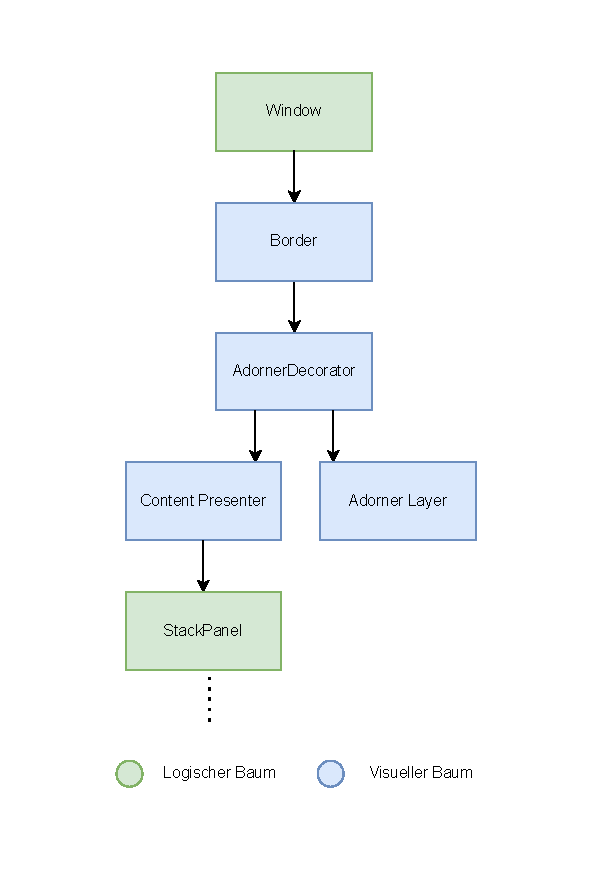
\includegraphics[width=0.5\textwidth]{4_Logical_Visual_Tree}
    \caption{Visueller und logischer Elementbaum}
    \label{fig:logical_visual_tree}
\end{figure}

\section{AssemblyResolver}
\label{sec:assembly_resolver}
Für die Konfiguration in Abschnitt \ref{sec:configuration_concept} müssen bestimmte Assemblies (siehe Unterabschnitt \ref{subsec:assemblies}) gefunden werden, die Klassen enthalten, welche ein bestimmtes Interface implementieren.

Da dies insbesondere bei größeren Anwendungen zu Performanceproblemen führen kann, werden alle relevanten Assemblies bereits während des Build-Prozesses auf die Implementierung entsprechender Interfaces überprüft. Die dabei gefundenen Assemblies werden anschließend registriert und in einem Zwischenspeicher abgelegt.

Bei späteren Suchvorgängen nach Klassen, die ein bestimmtes Interface implementieren, müssen dadurch nicht mehr alle Assemblies durchsucht werden, sondern nur diejenigen, die tatsächlich relevant sind. Dies reduziert den Suchaufwand und verbessert die Ladezeit der Anwendung.